\section{Introduction to R}

\begin{frame}{What is R?}
  \begin{minipage}{.675\textwidth}
  \begin{itemize}[<+-|alert@+>]
    \item \emph{lingua franca} for statistical computing and data analytics.
    \item Part programming language, part data analysis package.
  \end{itemize}
  \end{minipage}
  \hfill
  \begin{minipage}{.3\textwidth}
    \centering
\includegraphics[scale=.85]{../common/pics/Rlogo}
  \end{minipage}
  \begin{itemize}
    \item Dialect of S (1976, Bell Labs).
    \item Free (GPL $\geq 2$)
    \item A C program (mostly): 52\% C, 26\% Fortran, 22\% R
    \item Highly extensible; has over 7000 user-contributed packages.
  \end{itemize}
\end{frame}

\begin{frame}{R Continues to Move Up in Popularity!}
\vspace{-2em}
  \begin{center}
    IEEE Spectrum's 2015 Ranking of Programming Languages\\[1ex]
    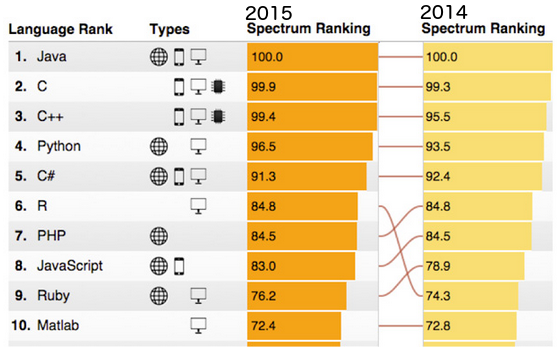
\includegraphics[scale=.45]{../common/pics/IEEE_Spectrum_Rank.png}
  \end{center}
  \vspace{-3em}
 {\scriptsize
\url{%
http://spectrum.ieee.org/computing/software/the-2015-top-ten-programming-languages
}}
\end{frame}


\begin{frame}
  \begin{block}{Resources for Learning R}\pause
  \begin{itemize}[<+-|alert@+>]
    \item \emph{The Art of R Programming} by Norm Matloff:
\url{http://nostarch.com/artofr.htm}\\[.2cm]

    \item \emph{An Introduction to R} by Venables, Smith, and the R Core Team:
\url{http://cran.r-project.org/doc/manuals/R-intro.pdf}\\[.2cm]

    \item \emph{The R Inferno} by Patrick Burns:
\url{http://www.burns-stat.com/pages/Tutor/R_inferno.pdf}\\[.2cm]

    \item Mathesaurus:  \url{http://mathesaurus.sourceforge.net/}\\[.2cm]

    \item R programming for those coming from other languages:
\url{http://www.johndcook.com/R_language_for_programmers.html}\\[.2cm]

    \item \emph{aRrgh: a newcomer's (angry) guide to R}, by Tim Smith and Kevin
Ushey:
    \url{http://tim-smith.us/arrgh/}
    \item \emph{Advanced R}: \url{http://adv-r.had.co.nz} by Hadley Wickham
    \item \emph{Grammar of Graphics}: \url{http://ggplot2.org} by Hadley Wickham
  \end{itemize}
\end{block}
\end{frame}


\begin{frame}
  \begin{block}{Other Invaluable Resources}\pause
    \begin{itemize}[<+-|alert@+>]
    \item \emph{R Installation and Administration}:
      \url{http://cran.r-project.org/doc/manuals/R-admin.html}
    \item \emph{Task Views}:
      \url{http://cran.at.r-project.org/web/views}
    \item \emph{Writing R Extensions}:
      \url{http://cran.r-project.org/doc/manuals/R-exts.html}
    \item Mailing list archives: \url{http://tolstoy.newcastle.edu.au/R/}
    \item The \code{[R]} stackoverflow tag.
    \end{itemize}
  \end{block}
\end{frame}



